\documentclass{article}

\usepackage[margin=0.5in]{geometry}
\usepackage{multicol}
\usepackage{siunitx}
\usepackage{enumitem}
\usepackage{graphicx}

\title{Polygons Lecture Problems}
\author{}
\date{}

\begin{document}
\maketitle
\begin{enumerate}
    \item What is the area of trapezoid $ABCD$?
        \begin{center}
            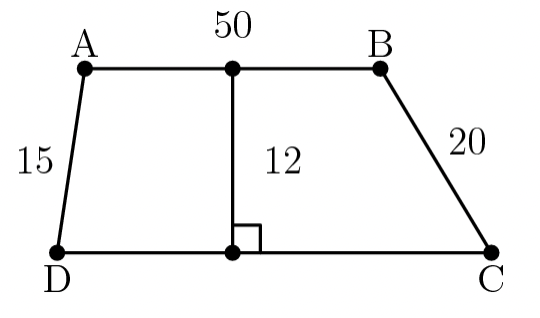
\includegraphics[scale=0.6]{trapezoid2.png}
        \end{center}
        \vspace{1cm}
    \item What is the smallest angle which can be created by connecting three vertices of a regular $36$-gon?
        \vspace{3cm}
    \item Find the length $AC$ in the regular hexagon $ABCDEF$ if the perimeter of the hexagon is $24$ cm.
        \vspace{3cm}
    \item Regular octagon $ABCDEFGH$ has side length $2$ centimeters.
        Find the area of square $ACEG$.
\end{enumerate}
\end{document}


